% !TEX root = ../../prj4projektdokumentation.tex
% SKAL STÅ I TOPPEN AF ALLE FILER FOR AT MASTER-filen KOMPILERES 

\section{Blok definitionsdiagram}
Et BDD for spændingsregulator ses på figur \ref{fig:BDDSpaendingsregulator}. På diagrammet ses de overordnet blokke spædingsregulator består af. En beskrivelse af hver blok kan læses under figur \ref{fig:BDDSpaendingsregulator}.

\begin{figure}[htbp] % (alternativt [H])
	\centering
	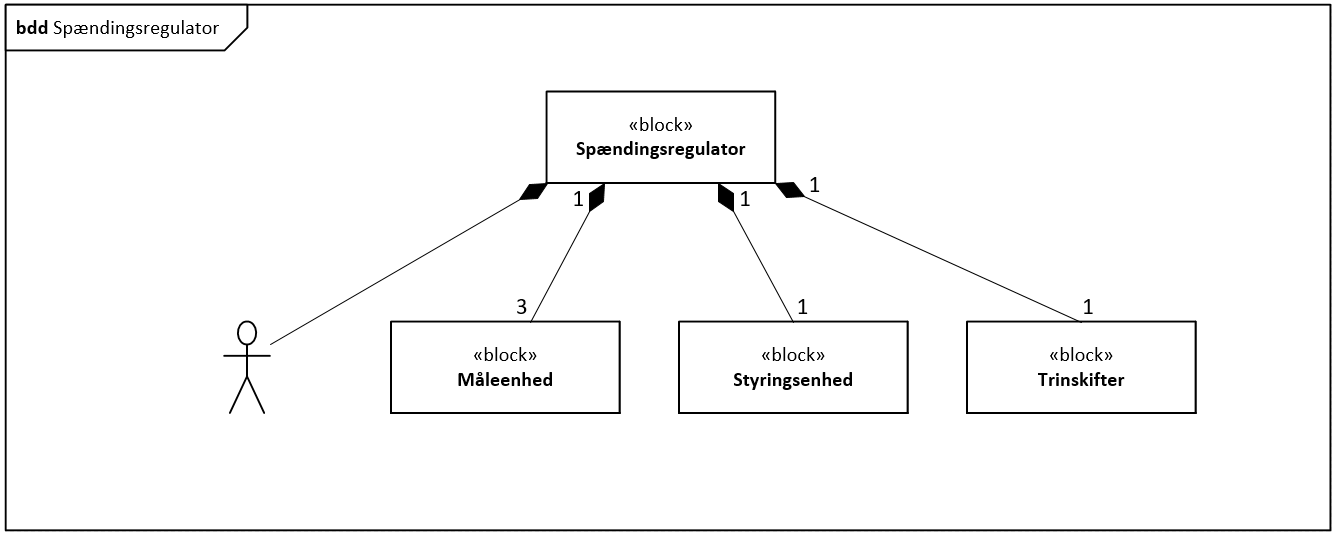
\includegraphics[width=0.9\textwidth]{Figure/BDDSpaendingsregulator}
	\caption{BDD Spaendingsregulator}
	\label{fig:BDDSpaendingsregulator}
\end{figure}

\textbf{Forbruger måleenhed} står for at måle spænding, strøm og faseforskydningen herimellem. Den består af nogle modstande og en PSoC 5. ?? På enheden ligger også noget af behandlingen af rådataet, så dette kan formidles til styringsenheden.

\textbf{Central målenehed} skal kunne måle spænding, strøm, faseforskydningen herimellem og indeholdet af harmoniske frekvenser. Den består af en PSoC 5 og hardware til måling af de nævnte parametre. Ligesom Forbruger måleenheden skal den kunne formidle dataet til styringsenheden.

\textbf{Styringsenhed} har til opgave at styre trinskifteren ud fra de data den får fra Forburger måleenheden og Central måleenheden. Den består af en PLC.....

\textbf{Trinskifter}